\chapter*{Introduzione}
\addcontentsline{toc}{chapter}{\numberline{}Introduzione}
\begin{flushright}
\enf{L'anima mia attende il Signore\\
Pi\`u che le sentinelle l'aurora.}
\end{flushright}

Questa dispensa \`e nata come pretesto per affinare le mie capacit\`a
con \LaTeX. Penso di aver raggiunto il mio scopo.

Era mia intenzione distribuirla gratuitamente, e per un periodo di tempo
\`e stato cos\`i. Poi cambiai opinione, e decisi di lavoravici per poi
venderla al prezzo di due pacchetti di Marlboro.

Voi che leggete non l'avete pagata, quindi ho evidentemente cambiato di
nuovo idea. Perch\'e? Be', i motivi sono tanti, il principale dei quali
\`e, probabilmente, la filosofia che sta dietro all'open source, motivo
per il quale ora, non solo la dispensa \`e gratuita, ma \`e anche
disponibile il suo codice sorgente (non azzardatevi a cambiare questa
pagina \ldots)

\begin{wrapfigure}[10]{r}{4cm}
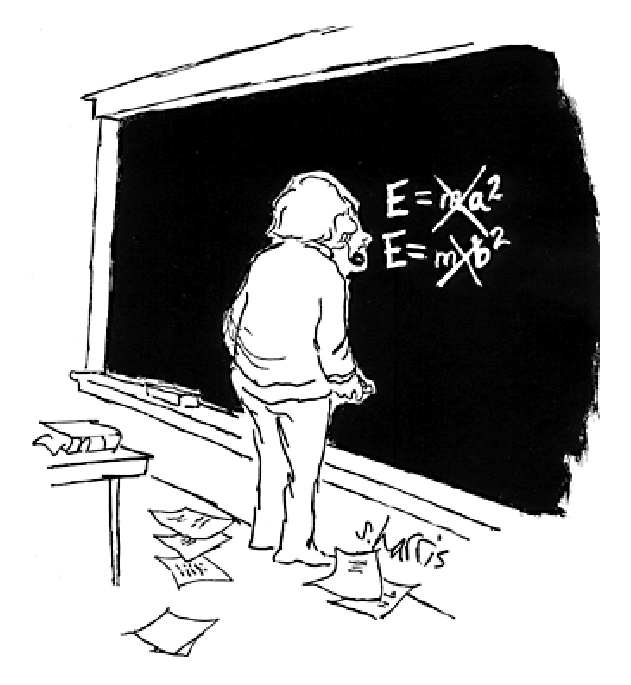
\includegraphics[width=3cm]{emcsquaredcartoon.eps}
\end{wrapfigure}

Ringrazio Alessandro Broggio per l'aiuto datomi nella stesura di questa
dispensa, il professor Zampieri e il professor Zilio, che m'hanno
accompagnato, chi pi\`u, chi meno, nel mondo della matematica e della
fisica, alle scuole superiori; inoltre ringrazio il professor Marchetti,
che s'\`e preoccupato di correggermi la dispensa, di fare la tesi con
me, e di tenere il corso, nonch\'e di favorire noi studenti di fronte ai
professori di laboratorio del C.C.S. di fisica, che cercano sempre di
rubare ore alle materie pi\`u belle. Il ringraziamento pi\`u grande va
poi a Giuditta, senza la quale non avrei scritto niente, essendo stata
lei a spingermi a continuare quando di voglia non ne avevo.

V'\`e poi la mia mail \emph{lanzani@spiro.fisica.unipd.it},\footnote{Ho
una ragazza, studio, sono in Erasmus in Olanda, da dove,
spero, non torner\`o: quindi non ho tutto il tempo libero che avete voi:
pazientate se non vi rispondo subito.} attiva per ricevere suggerimenti
che vi vengono alla mente, ed errori che riscontrate, nella lettura di
questa dispensa. \`E anche stata messa sotto cvs, ma la cosa non mi pare
abbia riscosso troppo successo, in quanto oltre a me nessuno l'ha mai
modificata. In ogni caso la potete trovare, coi sorgenti, su
\begin{center}
	http://spiro.fisica.unipd.it/$\thicksim$lanzani/public/rel/
\end{center}

 Una nota per tutti i computer nerd con mille suggerimenti stilistici:
cercate di concentrare le vostre energie nel correggere la ``sostanza''
della dispensa.

Parlando del corso: non preoccupatevi per la notazione tensoriale: sarebbero
necessari esercizi semplici per impratichirsi. Il resto \`e tutto
abbastanza facile, e, soprattutto bello. Forse potr\`a risultare ancora
pi\`u interessante leggere la mia tesi di laurea, che costituisce la
seconda parte della dispensa. Non \`e molto difficile, e penso che una
volta terminato il corso (ma anche prima), sarete perfettamente in grado
di apprezzarne il valore.

Il corso si conclude con un'ora di relativit\`a generale, durante la quale,
ovviamente, non s'\`e nemmeno avuto il tempo di farsi una vaga
idea di quello che \`e la relativit\`a generale, e perci\`o non la
riporto.

 \vskip 0.2cm
 \hskip 1cm Giovanni Lanzani
